% Options for packages loaded elsewhere
% Options for packages loaded elsewhere
\PassOptionsToPackage{unicode}{hyperref}
\PassOptionsToPackage{hyphens}{url}
%
\documentclass[
  ignorenonframetext,
  english,
]{beamer}
\newif\ifbibliography
\usepackage{pgfpages}
\setbeamertemplate{caption}[numbered]
\setbeamertemplate{caption label separator}{: }
\setbeamercolor{caption name}{fg=normal text.fg}
\beamertemplatenavigationsymbolsempty
% remove section numbering
\setbeamertemplate{part page}{
  \centering
  \begin{beamercolorbox}[sep=16pt,center]{part title}
    \usebeamerfont{part title}\insertpart\par
  \end{beamercolorbox}
}
\setbeamertemplate{section page}{
  \centering
  \begin{beamercolorbox}[sep=12pt,center]{section title}
    \usebeamerfont{section title}\insertsection\par
  \end{beamercolorbox}
}
\setbeamertemplate{subsection page}{
  \centering
  \begin{beamercolorbox}[sep=8pt,center]{subsection title}
    \usebeamerfont{subsection title}\insertsubsection\par
  \end{beamercolorbox}
}
% Prevent slide breaks in the middle of a paragraph
\widowpenalties 1 10000
\raggedbottom
\AtBeginPart{
  \frame{\partpage}
}
\AtBeginSection{
  \ifbibliography
  \else
    \frame{\sectionpage}
  \fi
}
\AtBeginSubsection{
  \frame{\subsectionpage}
}
\usepackage{iftex}
\ifPDFTeX
  \usepackage[T1]{fontenc}
  \usepackage[utf8]{inputenc}
  \usepackage{textcomp} % provide euro and other symbols
\else % if luatex or xetex
  \usepackage{unicode-math} % this also loads fontspec
  \defaultfontfeatures{Scale=MatchLowercase}
  \defaultfontfeatures[\rmfamily]{Ligatures=TeX,Scale=1}
\fi
\usepackage{lmodern}

\ifPDFTeX\else
  % xetex/luatex font selection
\fi
% Use upquote if available, for straight quotes in verbatim environments
\IfFileExists{upquote.sty}{\usepackage{upquote}}{}
\IfFileExists{microtype.sty}{% use microtype if available
  \usepackage[]{microtype}
  \UseMicrotypeSet[protrusion]{basicmath} % disable protrusion for tt fonts
}{}
\makeatletter
\@ifundefined{KOMAClassName}{% if non-KOMA class
  \IfFileExists{parskip.sty}{%
    \usepackage{parskip}
  }{% else
    \setlength{\parindent}{0pt}
    \setlength{\parskip}{6pt plus 2pt minus 1pt}}
}{% if KOMA class
  \KOMAoptions{parskip=half}}
\makeatother


\usepackage{longtable,booktabs,array}
\newcounter{none} % for unnumbered tables
\usepackage{calc} % for calculating minipage widths
\usepackage{caption}
% Make caption package work with longtable
\makeatletter
\def\fnum@table{\tablename~\thetable}
\makeatother
\usepackage{graphicx}
\makeatletter
\newsavebox\pandoc@box
\newcommand*\pandocbounded[1]{% scales image to fit in text height/width
  \sbox\pandoc@box{#1}%
  \Gscale@div\@tempa{\textheight}{\dimexpr\ht\pandoc@box+\dp\pandoc@box\relax}%
  \Gscale@div\@tempb{\linewidth}{\wd\pandoc@box}%
  \ifdim\@tempb\p@<\@tempa\p@\let\@tempa\@tempb\fi% select the smaller of both
  \ifdim\@tempa\p@<\p@\scalebox{\@tempa}{\usebox\pandoc@box}%
  \else\usebox{\pandoc@box}%
  \fi%
}
% Set default figure placement to htbp
\def\fps@figure{htbp}
\makeatother



\ifLuaTeX
\usepackage[bidi=basic,shorthands=off]{babel}
\else
\usepackage[bidi=default,shorthands=off]{babel}
\fi
\ifLuaTeX
  \usepackage{selnolig} % disable illegal ligatures
\fi


\setlength{\emergencystretch}{3em} % prevent overfull lines

\providecommand{\tightlist}{%
  \setlength{\itemsep}{0pt}\setlength{\parskip}{0pt}}



 


\makeatletter
\@ifpackageloaded{caption}{}{\usepackage{caption}}
\AtBeginDocument{%
\ifdefined\contentsname
  \renewcommand*\contentsname{Table of contents}
\else
  \newcommand\contentsname{Table of contents}
\fi
\ifdefined\listfigurename
  \renewcommand*\listfigurename{List of Figures}
\else
  \newcommand\listfigurename{List of Figures}
\fi
\ifdefined\listtablename
  \renewcommand*\listtablename{List of Tables}
\else
  \newcommand\listtablename{List of Tables}
\fi
\ifdefined\figurename
  \renewcommand*\figurename{Figure}
\else
  \newcommand\figurename{Figure}
\fi
\ifdefined\tablename
  \renewcommand*\tablename{Table}
\else
  \newcommand\tablename{Table}
\fi
}
\@ifpackageloaded{float}{}{\usepackage{float}}
\floatstyle{ruled}
\@ifundefined{c@chapter}{\newfloat{codelisting}{h}{lop}}{\newfloat{codelisting}{h}{lop}[chapter]}
\floatname{codelisting}{Listing}
\newcommand*\listoflistings{\listof{codelisting}{List of Listings}}
\makeatother
\makeatletter
\makeatother
\makeatletter
\@ifpackageloaded{caption}{}{\usepackage{caption}}
\@ifpackageloaded{subcaption}{}{\usepackage{subcaption}}
\makeatother

\usepackage{bookmark}
\IfFileExists{xurl.sty}{\usepackage{xurl}}{} % add URL line breaks if available
\urlstyle{same}
\hypersetup{
  pdftitle={ECN 102: Analysis of Economics Data},
  pdfauthor={Remy Beauregard},
  pdflang={en},
  hidelinks,
  pdfcreator={LaTeX via pandoc}}


\title{\texorpdfstring{ECN 102: Analysis of Economics
Data}{ECN 102: Analysis of Economics Data}}
\subtitle{\texorpdfstring{Chapter 6: The Least Squares
Estimator}{Chapter 6: The Least Squares Estimator}}
\author{Remy Beauregard}
\date{}

\begin{document}
\frame{\titlepage}


\begin{frame}{Introduction to the Population Model}
\protect\phantomsection\label{introduction-to-the-population-model}
Previously, we have estimated a regression line for our sample of data,
\(\hat{y}=b_1+b_2x\). However, we want to use this sample estimation to
say something about the larger (unobserved) population our sample comes
from.

Typically, we are interested in learning about the slope coefficient
\(b_2\): how \(Y\) changes when \(X\) changes. To do this, we need to
impose more structure onto our bivariate regression analysis.
\end{frame}

\begin{frame}{Conditional Mean and Conditional Values of Y}
\protect\phantomsection\label{conditional-mean-and-conditional-values-of-y}
We wish to model the true population relationship between X and Y, what
we could estimate if we could observe the entire population. Doing this
would let us calculate \(\boldsymbol{E[Y|X=x]}\), the \emph{conditional
expected value of Y}, for each value of X.

We would also be able to observe \(\boldsymbol{Y|X=x}\), the
\emph{conditional values of Y} for each value of X.
\end{frame}

\begin{frame}{Population Model: Linearity Assumption}
\protect\phantomsection\label{population-model-linearity-assumption}
The first structure we put on our bivariate linear regression is that
the conditional expected value of Y (or conditional mean) is equal to:
\[E[Y|X=x] = \beta_1+\beta_2x\]

This assertion means that the relationship between X and Y is truly
linear and that our sample estimates \(b_1,b_2\) are estimators for
\(\beta_1,\beta_2\).
\end{frame}

\begin{frame}{The Error Term in the Population Model}
\protect\phantomsection\label{the-error-term-in-the-population-model}
Just like our sample regression line, we do not assume that X can always
perfectly predict Y (or, that our data points always lie on the line
\(\beta_1+\beta_2x\)). Instead, we introduce an \textbf{error term} into
the above regression, to allow noise in our population relationship:

\[E[Y|X=x]=\beta_1+\beta_2x+\boldsymbol{u}\]

Importantly, however, this error term is not a \emph{residual} that we
aim to minimize --- it is the \emph{true noise or disturbance} in the
relationship between X and Y. Like our true population model, this true
error term is unobserved.
\end{frame}

\begin{frame}{Zero Conditional Mean of the Error Term}
\protect\phantomsection\label{zero-conditional-mean-of-the-error-term}
For any individual value of X, we assume that our error term may be
positive or negative. In expectation, however, we assume that the
conditional mean of the error is zero:

\[E[u|x]=0\]

Alternatively, this means we are assuming:

\[E[y|x]=\beta_1+\beta_2x\]
\end{frame}

\begin{frame}{Graphical Representation: Y\textbar X
vs.~E{[}Y\textbar X{]}}
\protect\phantomsection\label{graphical-representation-yx-vs.-eyx}
\begin{figure}

\centering{

\pandocbounded{\includegraphics[keepaspectratio,alt={Scatter plot illustrating the population regression model. A line labeled β₁+β₂x passes through the conditional mean E{[}Y\textbar X=x{]} (diamond marker) at the value X=x. Individual conditional values Y\textbar X are scattered as dots around the line. At the highlighted value X=x, a dashed vertical line separates points above the line, labeled u greater than 0, from points below it, labeled u less than 0, showing that the error term u is the deviation of each Y\textbar X observation from its conditional mean.}]{L6_files/figure-beamer/fig-cond-values-1.pdf}}

}

\caption{\label{fig-cond-values}Population regression model}

\end{figure}%
\end{frame}

\begin{frame}{Variance of Y\textbar X and Homoskedasticity}
\protect\phantomsection\label{variance-of-yx-and-homoskedasticity}
Since \(u\) is the difference between \(Y\) and \(Y|X\), it follows that
\[Var[y|x]=Var[u|x]\]

In the simplest case, we assume that the variance of our error term
(``skedasticity'') is constant across all possible values of X:
\[\sigma^2_u=Var[u|x]\]

Constant errors across x we refer to as \textbf{homo}skedasticity.
Non-constant errors across x we call \textbf{hetero}skedasticity.
\end{frame}

\begin{frame}{Graphical Representation: Skedasticity}
\protect\phantomsection\label{graphical-representation-skedasticity}
\begin{columns}[T]
\begin{column}{0.5\linewidth}
\textbf{Homoskedasticity:}

\begin{figure}

\centering{

\pandocbounded{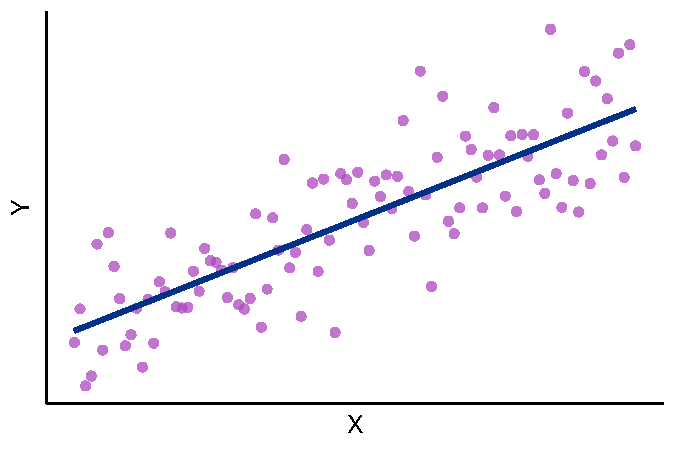
\includegraphics[keepaspectratio,alt={Scatter plot of Y against X illustrating homoskedasticity. A regression line runs through the data. The vertical spread of points around the line is roughly constant across all values of X, showing that error variance does not change with X.}]{L6_files/figure-beamer/fig-homo-1.pdf}}

}

\caption{\label{fig-homo}Homoskedastic data: constant error variance
across X}

\end{figure}%
\end{column}

\begin{column}{0.5\linewidth}
\textbf{Heteroskedasticity:}

\begin{figure}

\centering{

\pandocbounded{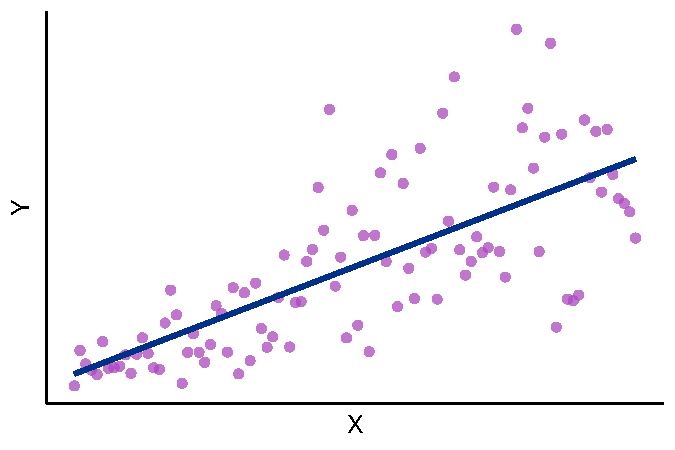
\includegraphics[keepaspectratio,alt={Scatter plot of Y against X illustrating heteroskedasticity. A regression line runs through the data. The vertical spread of points around the line grows larger as X increases, showing that error variance rises with X.}]{L6_files/figure-beamer/fig-hetero-1.pdf}}

}

\caption{\label{fig-hetero}Heteroskedastic data: error variance
increases with X}

\end{figure}%
\end{column}
\end{columns}
\end{frame}

\begin{frame}{Conditional Distribution of Y: Summary}
\protect\phantomsection\label{conditional-distribution-of-y-summary}
Taken together, these assumptions give us:
\[(Y|X=x_i)\sim(\beta_1+\beta_2x_i,\sigma^2_u)\]

``The random variable for conditional values \(Y|X=x_i\) is distributed
with population mean \(\beta_1+\beta_2x_i\) and population variance
\(\sigma^2_u\) (if I have errors that are constant across x and
conditional mean zero)''.
\end{frame}

\begin{frame}{Four Assumptions for Linear Regression}
\protect\phantomsection\label{four-assumptions-for-linear-regression}
We can formalize these \textbf{four assumptions for linear regression:}

\begin{enumerate}
[1)]
\item
  \textbf{Linearity:} our true population model is linear in X

  The population model is \(y_i=\beta_1+\beta_2x_i+u_i\) for all \(i\)
\end{enumerate}

\pause

\begin{enumerate}
[1)]
\setcounter{enumi}{1}
\item
  \textbf{Unbiasedness:} the conditional mean of the error term is zero

  \(E[u_i|x_i]=0\) for all \(i\)
\end{enumerate}

\pause

\begin{enumerate}
[1)]
\setcounter{enumi}{2}
\item
  \textbf{Homoskedasticity:} error term has constant variance across
  \(X\)

  \(Var[u_i|x_i]=\sigma^2_u\) for all \(i\)
\end{enumerate}

\pause

\begin{enumerate}
[1)]
\setcounter{enumi}{3}
\item
  \textbf{Independence:} error terms for different observations do not
  affect each other

  \(u_i \perp \!\!\! \perp u_j\) for all \(i\neq j\)
\end{enumerate}
\end{frame}

\begin{frame}{What the Four Assumptions Give Us}
\protect\phantomsection\label{what-the-four-assumptions-give-us}
What can we do with these assumptions?

Assumptions (1) + (2) allow us to say that \(E[b_2]=\beta_2\).

Assumptions (3) + (4)\footnote<\value{beamerpauses}->[frame]{and some
  algebra} allow us to say that
\(\sigma^2_{b_2}=\frac{\sigma^2_u}{\sum_{i=1}^n(x_i-\bar{x})^2}\)

Finally, our CLT says that our computed statistic will be normally
distributed whenever \(n>30\).
\end{frame}

\begin{frame}{Asymptotic Normality of the OLS Estimator}
\protect\phantomsection\label{asymptotic-normality-of-the-ols-estimator}
All together, these assumptions give us:

\[b_2\sim N(\beta_2,\sigma^2_{b_2})\text{ with }n>30\]

Standardizing \(b_2\) yields:

\[\frac{b_2-\beta_2}{\sigma_{b_2}}\sim N(0,1)\]

\(b_2\) is asymptotically normally distributed, just like we showed for
\(\bar{x}\). Like with our standardized \(\bar{x}\), we can now do
hypothesis testing on our estimated \(b_2\) coefficient.
\end{frame}

\begin{frame}{Unbiasedness and Consistency of OLS}
\protect\phantomsection\label{unbiasedness-and-consistency-of-ols}
We can claim that our OLS estimator \(b_2\) is both \emph{unbiased} and
\emph{consistent} under these four population assumptions:
\[\underbrace{E[b_2]=\beta_2}_{\text{Unbiased}}\text{ and }\underbrace{\sigma^2_{b_2}=\frac{\sigma^2_u}{\sum_{i=1}^{\boldsymbol{n}}(x_i-\bar{x})^2}\rightarrow0\text{ as }n\rightarrow\infty}_{\text{Consistent}}\]

\begin{figure}

\centering{

\pandocbounded{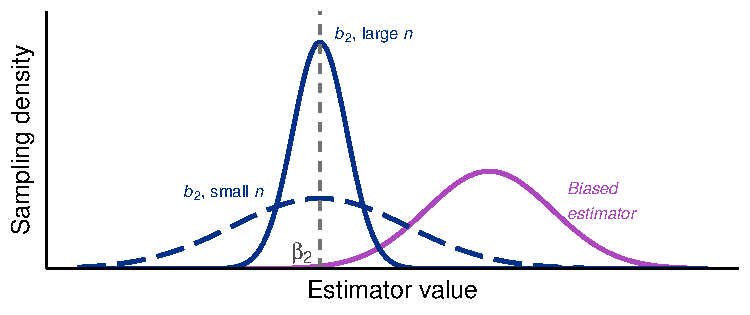
\includegraphics[keepaspectratio,alt={Density plot showing three bell-shaped sampling distribution curves. Two blue curves are centered at β₂, the true parameter value marked by a dashed vertical line: a wide, flat long-dashed curve for the OLS estimator at small n, and a tall, narrow solid curve for OLS at large n, illustrating that OLS is unbiased at all sample sizes and consistent as n increases. A purple curve centered to the right of β₂ represents a biased estimator whose distribution does not converge to the true value. The horizontal axis shows the estimator value and the vertical axis shows sampling density.}]{L6_files/figure-beamer/fig-ols-properties-1.pdf}}

}

\caption{\label{fig-ols-properties}Sampling distributions of the OLS
estimator \(b_2\) (unbiased and consistent) versus a biased estimator}

\end{figure}%
\end{frame}

\begin{frame}{OLS is BLUE: Best Linear Unbiased Estimator}
\protect\phantomsection\label{ols-is-blue-best-linear-unbiased-estimator}
We also call OLS \textbf{BLUE}: the \textbf{Best Linear Unbiased
Estimator}:

\begin{itemize}
\item
  \textbf{best} means that OLS has the minimum variance of all
  estimators in its class (not
  proven\footnote<\value{beamerpauses}->[frame]{If you are curious how
    we would show this, we use something called the \textbf{Gauss-Markov
    theorem} to show any other estimator would have higher variance.} in
  class)
\item
  \textbf{linear} means our assumed population model that we are
  estimating is linear
\item
  \textbf{unbiased} means our conditional error term is mean zero
\item
  \textbf{estimator} because we are estimating \(\beta_2\) with \(b_2\)
\end{itemize}
\end{frame}

\begin{frame}{Standard Error of the Slope Coefficient}
\protect\phantomsection\label{standard-error-of-the-slope-coefficient}
Since we do not actually observe \(u\) and thus do not know
\(\sigma^2_u\), however, we replace \(\sigma^2_u\) with \(s^2_e\) and
take a square root to get:
\[s_{b_2}=\frac{s_e}{\sqrt{\sum_{i=1}^n(x_i-\bar{x})^2}}\]

This is our \emph{standard error} of \(b_2\), an estimator for the
unknown population standard deviation of \(b_2\). Notice this uses
\(s_e\), the standard error of our residual/regression or RMSE, in its
numerator, meaning our model fit has a direct impact on the precision of
our estimator \(b_2\).
\end{frame}

\begin{frame}{Precision of the Slope Estimator}
\protect\phantomsection\label{precision-of-the-slope-estimator}
Given our standard error for \(b_2\) above, we observe circumstances
under which our slope coefficient \(\beta_2\) will be more precisely
estimated (or when our standard error of \(b_2\) will be smaller):
\[s_{b_2}=\frac{s_e}{\sqrt{\sum_{i=1}^n(x_i-\bar{x})^2}}\]

\begin{enumerate}
\item
  When our model fits better (\(s_e\) decreases) \(\Rightarrow\) numer.
  \(\downarrow\)
\item
  When our sample size (\(n\)) increases \(\Rightarrow\) denom.
  \(\sum_{i=1}^n \uparrow\)
\item
  When our regressor is more widely scattered/spread out relative to its
  mean \(\Rightarrow\) denom. \(\sum_i(x_i-\bar{x})^2\uparrow\)
\end{enumerate}
\end{frame}

\begin{frame}{Graphical Representation: Scattered vs.~Clustered Data}
\protect\phantomsection\label{graphical-representation-scattered-vs.-clustered-data}
\begin{columns}[T]
\begin{column}{0.5\linewidth}
\textbf{Clustered regressors} (imprecise):

\begin{figure}

\centering{

\pandocbounded{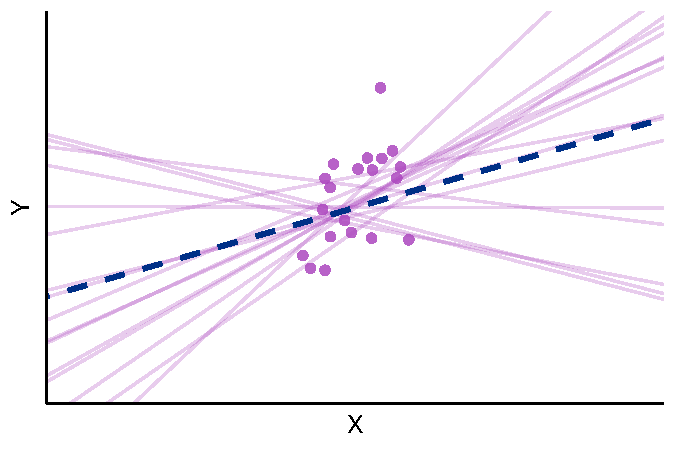
\includegraphics[keepaspectratio,alt={Scatter plot of Y against X where all data points are clustered in a narrow band of X values near the center of the horizontal axis. Many plausible regression lines are drawn through the cluster as a fan, showing that the slope coefficient b₂ can take a wide range of values --- illustrating high estimation imprecision when the regressor has little spread.}]{L6_files/figure-beamer/fig-slope-clustered-1.pdf}}

}

\caption{\label{fig-slope-clustered}Slope estimates from clustered X
data}

\end{figure}%
\end{column}

\begin{column}{0.5\linewidth}
\textbf{Scattered regressors} (precise):

\begin{figure}

\centering{

\pandocbounded{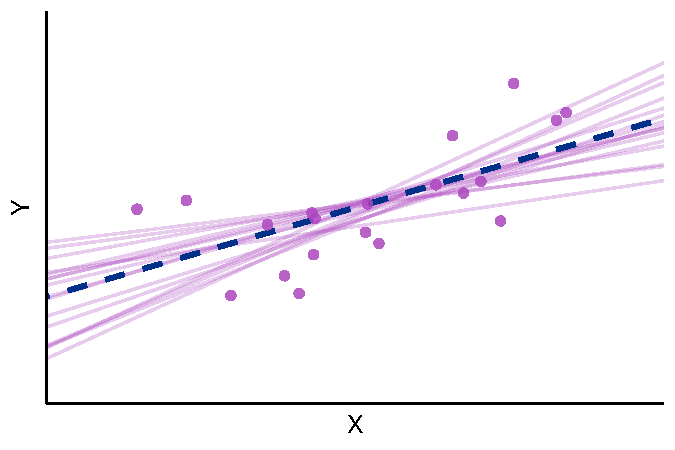
\includegraphics[keepaspectratio,alt={Scatter plot of Y against X where data points are spread widely across the full range of X values. Many regression lines are drawn through the data as a fan, but they are tightly clustered together, showing that the slope coefficient b₂ is estimated precisely when the regressor is widely spread. The true population regression line is shown as a blue dashed line.}]{L6_files/figure-beamer/fig-slope-spread-1.pdf}}

}

\caption{\label{fig-slope-spread}Slope estimates from spread-out X data}

\end{figure}%
\end{column}
\end{columns}
\end{frame}

\begin{frame}{Threats to the Regression Assumptions}
\protect\phantomsection\label{threats-to-the-regression-assumptions}
How can we deal with threats to these four population regression
assumptions? Do our statistics fall apart if these fail?
\end{frame}

\begin{frame}{Assumption Violation 1: Linearity}
\protect\phantomsection\label{assumption-violation-1-linearity}
\begin{enumerate}
\tightlist
\item
  Linearity is violated:
\end{enumerate}

Nonlinearity can be accommodated by least squares regressions to allow
for quadratic or other such relationships. This will affect \emph{how}
we estimate our coefficients but will not shut down estimation. We will
see examples of fitting nonlinear sample regression models in later
chapters, such as \(\hat{y}=b_1+b_2x+b_3x^2\) or a \emph{quadratic}
model.
\end{frame}

\begin{frame}{Assumption Violation 2: Unbiasedness}
\protect\phantomsection\label{assumption-violation-2-unbiasedness}
\begin{enumerate}
\setcounter{enumi}{1}
\tightlist
\item
  Unbiasedness is violated:
\end{enumerate}

Bias is a serious problem for estimation and requires careful
consideration to tackle properly. We say that a regression is biased
when its error term is correlated with its regressor:
\(Cov[u_i,x_i]\neq0\). We can try to get around this by adding missing
variables into the regression, or changing our regression specification
around this bias, but this remains a concern.
\end{frame}

\begin{frame}{Assumption Violation 3: Homoskedasticity}
\protect\phantomsection\label{assumption-violation-3-homoskedasticity}
\begin{enumerate}
\setcounter{enumi}{2}
\tightlist
\item
  Homoskedasticity is violated:
\end{enumerate}

Heteroskedasticity, or errors that vary in magnitude with x, can be
accommodated by using \textbf{robust standard errors}. This is a
relatively easy correction in Stata (or any program) that adjusts our
residuals with the magnitude of \(X\) to avoid potential
heteroskedasticity.

You are not responsible for the robust standard error formula. Broadly,
however, we expect it to undo the problematic \(f(x)\) making our errors
heteroskedastic: \(f(x)\sigma^2_u\) (with \(f'(x)>0\) or \(f'(x)<0\))
\end{frame}

\begin{frame}{Assumption Violation 4: Independence}
\protect\phantomsection\label{assumption-violation-4-independence}
\begin{enumerate}
\setcounter{enumi}{3}
\tightlist
\item
  Independence is violated:
\end{enumerate}

Error dependence, or observations influencing the error term of other
observations, is common in times series models, where US GDP this year
is highly correlated with US GDP last year. We have relatively easy
methods to account for this \emph{autocorrelation}.

We also may see errors correlated across units of observation (in
cross-sectional or panel data) and will see a method in later chapters
for dealing with such error dependence. Like robust standard errors,
this will also be relatively simple to implement.
\end{frame}

\section{End of Lecture Material}\label{end-of-lecture-material}

\begin{frame}{Knowledge Check 6}
\protect\phantomsection\label{knowledge-check-6}
For the following pairs of scenarios, state for which you would expect
\(\beta_2\) to be \emph{more precisely estimated} and why:

\begin{enumerate}
[a)]
\item
  \(n=45\) vs.~\(n=100\)
\item
  The regressor ranges from 10 to 20 vs.~from 10 to 50
\item
  The standard error of the regression \(s_e=2\) vs.~\(s_e=9\)
\end{enumerate}
\end{frame}




\end{document}
